\begin{newpage}
  \section{Develop}
  \label{sec:develop}
    % TODO: AWS - Instanz spezifikationen (Leistung) Medium Instanz?
    % TODO: AWS - Server Test bzw Metriken?

    In diesem Kapitel soll der Entwicklungsprozess zum besseren Verständnis einigermaßen linear beschrieben werden, obwohl der eigentliche Ablauf nicht immer dieser Linearität entsprach. Zuerst soll erläutert werden, welches Prinzip hinter der Animation einzelner Vehicle entlang einer Polyline steht. Anschließend wird dieser Ansatz weiterentwickelt, bis die Animation von allen aktiven Trips auf einer Karte möglich ist. Dabei wurden verschiedene Optimierungsmaßnahmen ergriffen, um Probleme bezüglich der Performance zu beseitigen. Vor allem die zu verarbeitende Datenmenge, als auch das Verarbeiten und Optimieren von GTFS-Feeds, sind die Kernpunkte in diesem Kapitel. 

    \subsection{Anzeigen einer Polyline}
\label{sub:anzeigen_einer_polyline}
  Zu Beginn stellte sich die Frage, wie sich in kleinen Schritten an das komplexe Thema einer Live-Visualisierung herangetastet werden kann. Die erste Hürde ist die Animation von nur \textbf{einem} Vehicle entlang einer Polyline. Die Umsetzung dieses ersten Schrittes soll in diesem und den nächsten zwei Abschnitten \ref{sub:hinzufügen_der_stationen} und \ref{sub:animieren_eines_vehicles_durch_interpolation} erklärt werden.

  Um eine Datengrundlage zu haben, wurde ein möglichst vollständiges GTFS-Feed  ausgewählt\footnote{\url{http://TransitFeeds.com}} und in die Datenbank importiert. Die Wahl fiel dabei auf das Boston-MBTA Feed. Die Herausforderung bestand nun darin, erste Daten aus der Datenbank an den Client zu senden und sie dort darzustellen. Fast trivial ist das Abfragen der Polyline:

  \colorbox{lightGrey}{\texttt{\color{white}{{\color{materialBlue} SELECT} * {\color{materialBlue}FROM} gtfs\_shapes {\color{materialBlue}WHERE} shape\_id = {\color{materialRed}12345}}}}

  \begin{figure}[htbp]
    \begin{center}
      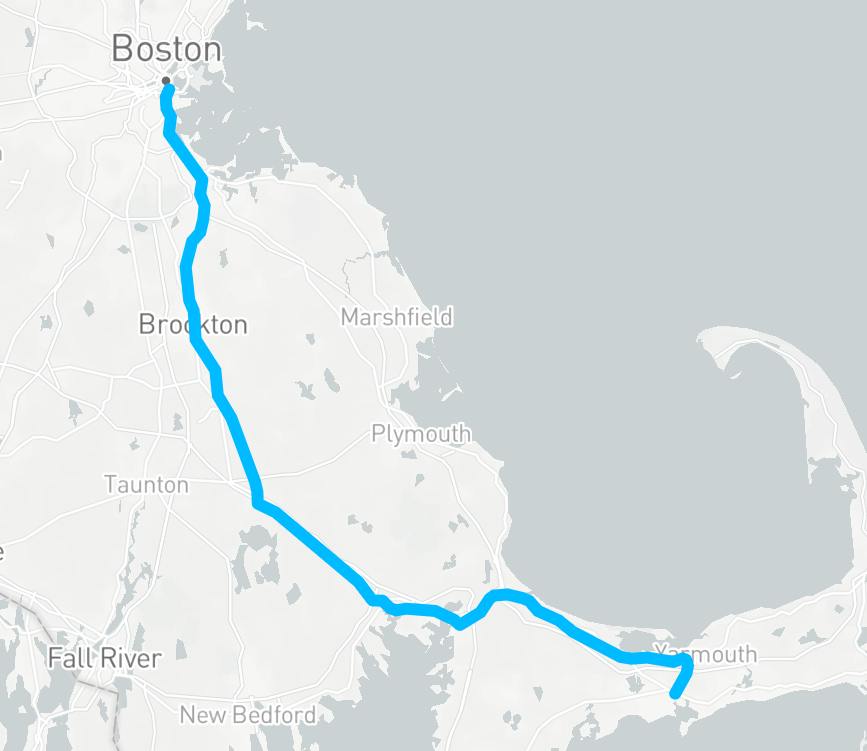
\includegraphics[width=0.5\textwidth]{prozess/draw_single_shape}
      \caption{Anzeigen einer einzigen Polyline in Boston}
      \label{fig:prozess/draw_single_shape}
    \end{center}
  \end{figure}
  
  Die Daten der Polyline werden als GeoJSON übertragen und lassen sich mittels Mapbox-gl-js auf der Karte anzeigen. Abbildung \ref{fig:prozess/draw_single_shape} zeigt das Ergebnis dieser ersten Iteration. Zu sehen ist bereits die Karte mit der Polyline (hier in blau). Die abgefragten Daten können nun also bereits verarbeitet und angezeigt werden. Damit ein Vehicle entlang dieser Linie animiert werden kann, werden die einzelnen Stationen des Trips benötigt.
  Dieser ständige Wechsel zwischen der Arbeit am Backend, um neue Datenabfragen zu ermöglichen und dem Frontend, um diese anschließend anzuzeigen, stellte sich als sehr effektiv heraus und zog sich durch das gesamte Projekt hinweg durch.
% subsection anzeigen_einer_polyline (end)
    \subsection{Hinzufügen der Stationen}
\label{sub:hinzufügen_der_stationen}
  Nachdem die Polyline auf die Karte gebracht wurde, werden die Stationen des Trips benötigt (Abbildung \ref{fig:prozess/add_stations}). Diese beinhalten für die Animation essentielle Daten wie zum Beispiel Abfahrts- und Ankunftszeit eines Vehicles. Die genaue SQL-Abfrage dafür soll an dieser Stelle der Einfachheit wegen ausgespart bleiben.

  \begin{figure}[htbp]
    \begin{center}
      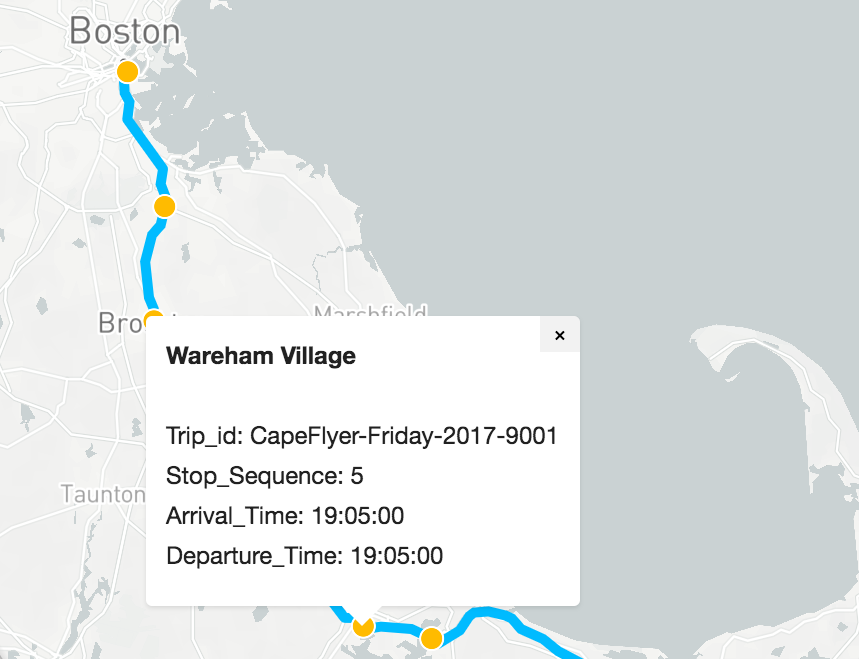
\includegraphics[width=0.5\textwidth]{prozess/add_stations}
      \caption{Hinzufügen von Stationen entlang der Polyline}
      \label{fig:prozess/add_stations}
    \end{center}
  \end{figure}

  Für die Animation der Vehicle (Abschnitt \ref{sub:animieren_eines_vehicles_durch_interpolation}) wird außerdem der Wert für die Differenz der \texttt{distance\_traveled}, also die Distanz zwischen den einzelnen Stationen, benötigt. Diese kann aus den distance\_traveled-Werten der einzelnen Stationen über Subtraktion berechnet werden. Nun hat zwar das Stuttgart-VVS-Feed ein distance\_traveled-Feld, welches die benötigten Distanz-Informationen direkt aus der Datenbank liefert; für andere GTFS-Feeds, die getestet wurden, ist dieses Feld jedoch oftmals nicht vorhanden. Aus diesem Grund wurde ein Algorithmus entwickelt, welcher über ein sogenanntes \texttt{Station-Matching} die Werte der distance\_traveled und damit die Distanz zwischen den Stationen ermitteln kann. Der Station-Matching-Algorithmus wird von der Applikation nur dann als Fallback-Lösung für die Berechnung verwendet, wenn das distance\_traveled-Feld nicht im Feed vorhanden ist.

  \subsubsection*{Station-Matching}
  \label{ssub:station_matching}
    Das Station-Matching soll folgendes Problem lösen:

    \begin{figure}[htbp]
      \begin{center}
        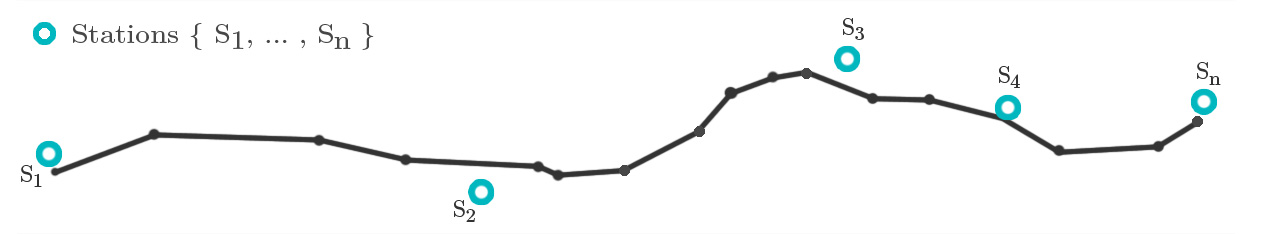
\includegraphics[width=\textwidth]{station_problem.jpg}
        \caption{Stationen liegen nicht direkt auf der Polyline}
        \label{fig:station_problem}
      \end{center}
    \end{figure}
    
    Wie in Abbildung \ref{fig:station_problem} zu sehen ist, sind die Stationen (Haltestellen oder Bahnhöfe) nicht exakt auf der Polyline, sondern ein wenig abseits positioniert, da dies auch ihrem realen Standort neben der Fahrbahn entspricht. Um nun die Distanzen zwischen den Stationen zu berechnen, legt der Algorithmus im Sinne des Matchings zunächst die Stationen auf die Polyline.  

    \begin{figure}[htbp]
      \begin{center}
        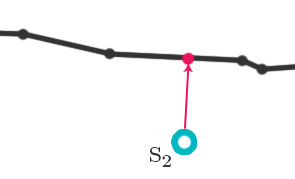
\includegraphics[width=0.25\textwidth]{find_nearest_point}
        \caption{Finde den nächstgelegenen Punkt der Station auf der Polyline}
        \label{fig:find_nearest_point}
      \end{center}
    \end{figure}

    Nachdem der entsprechende Punkt auf der Polyline gefunden wurde, berechnet der Algorithmus die jeweiligen Wegstrecken zur ersten Station des Trips (distance\_traveled), bevor er die Werte von aufeinanderfolgenden Stationen subtrahiert.  Die Distanz zweier Stationen $\{S_i,S_{i+1} \;|\; i \in \mathbb{N} \}$ sei $d_\triangle$. Diese kann jetzt wie folgt berechnet werden: $d_{\triangle_i} = d_{S_n} - d_{S_{n-1}}\;|\; d_S := DistanceTraveled, n \in \mathbb{N}, n \ge 2$ 
    In Listing \ref{lst:match_station} des Anhangs wird dieser Station-Matching-Algorithmus vorgestellt.

    \begin{figure}[htbp]
      \begin{center}
        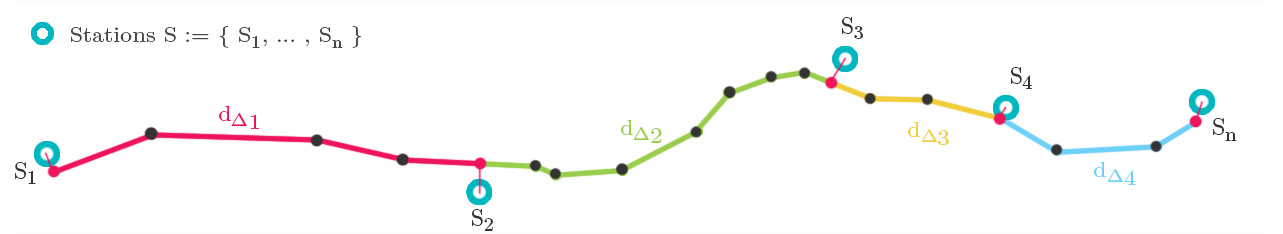
\includegraphics[width=\textwidth]{get_distances}
        \caption{Berechnen der Distanz}
        \label{fig:get_distances}
      \end{center}
    \end{figure}
    
    Abbildung \ref{fig:station_matching_comparision} stellt eine frühere Implementierung mit der nun aktuellen Version des Algorithmus gegenüber, indem die für das Matching über $n$-Trips benötigte Zeit der beiden Algorithmen verglichen wird. Um eine durchschnittliche Laufzeit zu erhalten, wurde jeder Algorithmus 10 mal mit der gleichen Anzahl an Trips ausgeführt.

    \begin{figure}[htbp]
      \begin{center}
        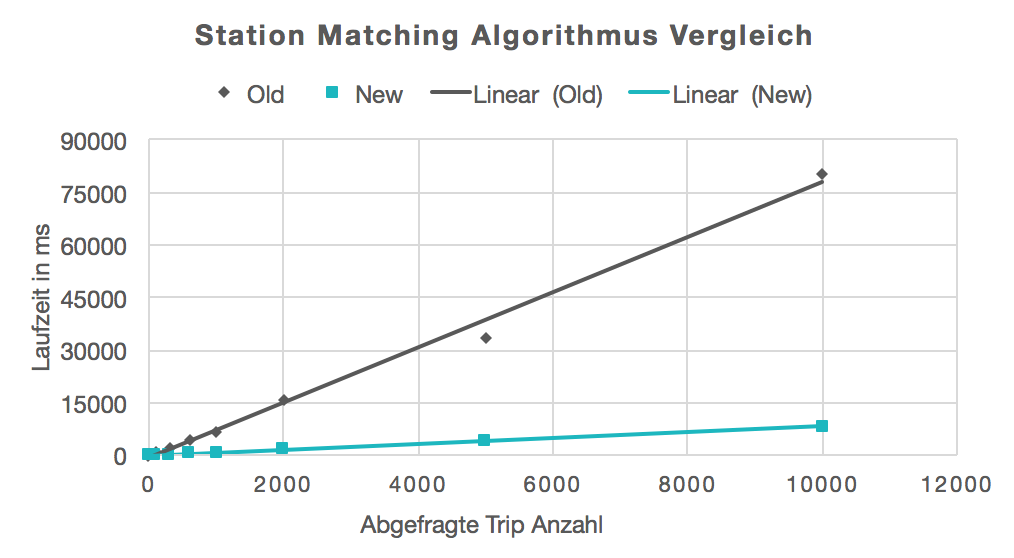
\includegraphics[width=0.7\textwidth]{station_matching_comparision}
        \caption{Vergleich der zwei Station-Matching-Algorithmen}
        \label{fig:station_matching_comparision}
      \end{center}
    \end{figure}

    Der alte Algorithmus war sehr simpel und beruhte darauf, die Funktion \texttt{pointOnLine} der \texttt{Turf.js}-Bibliothek zu verwenden. Diese Funktion hatte den entscheidenden Nachteil, dass sie in 3 \texttt{for}-Schleifen über die gesamten Punkte der Polyline iteriert. Hinzu kommt, dass das Matching nicht nur auf eine Station, sondern auf sämtliche Stationen aus allen Trips angewendet werden muss. Das führte dazu, dass insgesamt 5 \texttt{for}-Schleifen verwendet wurden. Damit lässt sich der im Vergleich höhere Anstieg der Laufzeit bei steigender Trip-Anzahl erklären. Generell ist der neue Algorithmus sehr viel schneller. Durch die Verwendung eines \texttt{R-Trees}\footnote{Ein R-Tree (R für Rectangle) bezeichnet eine baumförmige Datenstruktur für das Speichern und Abfragen von raumbezogenen Informationen. In Verwendung ist folgende Bibliothek: \url{https://github.com/mourner/rbush}} und der eigenen Implementierung verschiedener Bibliotheksfunktionen (turf.lineSlice, turf.pointOnLine), konnte die Laufzeit drastisch reduziert werden (siehe Tabelle \ref{tbl:station_matching_comparison}).

    \begin{longtable}{|>{\raggedright \arraybackslash}p{5.0cm}|>{\raggedright \arraybackslash}p{2.2cm}|>{\raggedright \arraybackslash}p{2.2cm}|}
    \caption{Station-Matching Vergleich Old / New}\label{tbl:station_matching_comparison}\\
      \hline
      Anz. verarbeiteter Trips & Old (in ms)& New (in ms)\\
      \hline
      100    & 712   & 121  \\
      300    & 2191  & 305  \\
      600    & 4344  & 545  \\
      1.000  & 6780  & 874  \\
      2.000  & 15782 & 1700 \\
      5.000  & 33708 & 4161 \\
      10.000 & 80291 & 8279 \\
      \hline
    \end{longtable}

    Zwar wachsen beide Implementierungen lediglich linear mit steigender Trip-Anzahl, allerdings benötigt der neue Algorithmus für die Verarbeitung von $10.000$ Trips anstatt $80.29$ nur $8.28$ Sekunden.  

    Im Realbetrieb verarbeitet der Server zwischen $0 - 500$ Trips. Bei dieser Anzahl beträgt die Laufzeit des Algorithmus $\approx80ms - 400ms$. Dadurch kann argumentiert werden, dass der Algorithmus gerade noch schnell genug für eine Webanwendung arbeitet. Auch größere Anzahlen an Trips wären noch in akzeptabler Geschwindigkeit berechenbar. So können $1000$ Trips immer noch in unter einer Sekunde berechnet werden. Allerdings wäre es bei einer größeren Anzahl an Trips ein falscher Ansatz, diese bei jeder Serveranfrage neu zu kalkulieren.

    \pagebreak

    Besser wäre es, einmalig das Matching für alle Trips eines GTFS-Feeds durchzuführen und die Ergebnisse persistent in der Datenbank abzuspeichern. Dies könnte beispielsweise gleich beim Importieren der Daten in die Datenbank geschehen. Dadurch könnte die Berechnung komplett eingespart werden. 
    Da für das Stuttgart-VVS-Feed glücklicherweise die zurückgelegte Distanz bis zu einer Station bereits zur Verfügung steht, muss nur noch die Distanz zwischen den Stationen ($d\triangle$) berechnet werden. Dies geschieht nach dem selben Prinzip wie in der oben genannten Subtraktions-Formel. Diese Berechnung ist trivial und erfolgt bei $10.000$ Trips in unter 15 Millisekunden.

  % subsubsection station_matching (end)
% subsection hinzufügen_der_stationen (end)
    \subsection{Animieren eines Vehicles durch Interpolation}
\label{sub:animieren_eines_vehicles_durch_interpolation}
  Der zentrale Kerngedanke für die Animation der Vehicle-Bewegung ist die Interpolation von Distanzen zwischen zwei aufeinanderfolgenden Stationen A und B mit der Distanz  $d_{\triangle}$. Um zu verstehen, wie ein Vehicle zwischen den einzelnen Stationen interpoliert werden kann, soll Abbildung \ref{fig:interpolating_vehicle} helfen.

  \begin{figure}[htbp]
    \begin{center}
      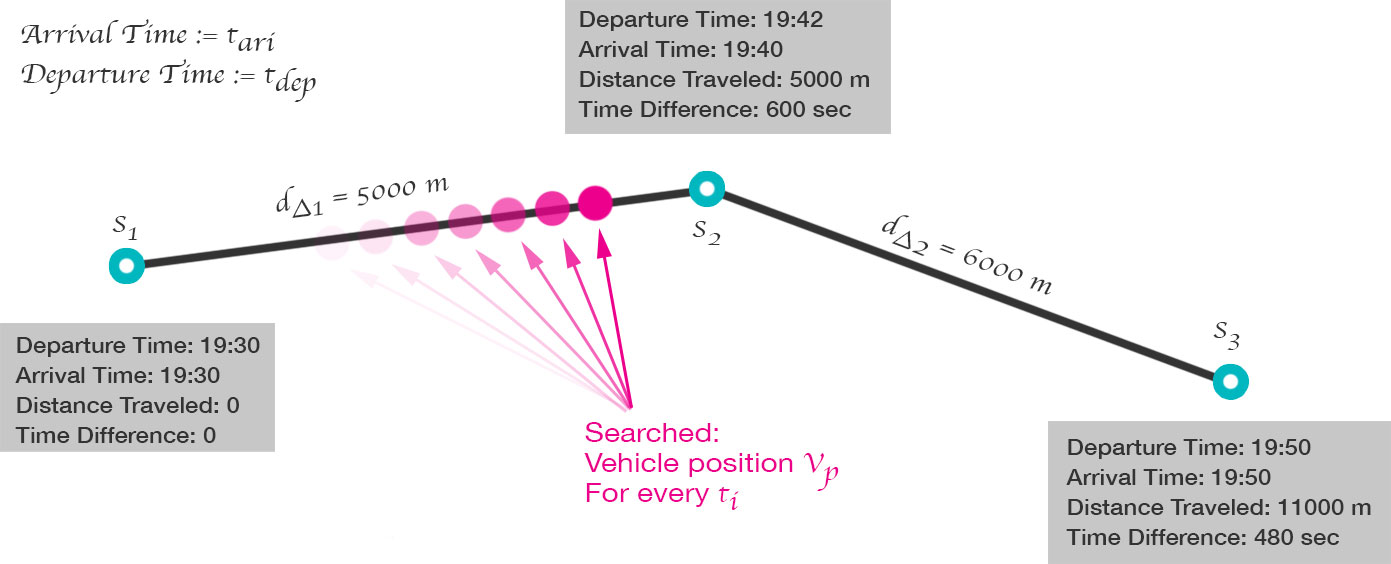
\includegraphics[width=0.9\textwidth]{interpolating_vehicle}
      \caption{Interpolation der Vehicle Position: $V_p$}
      \label{fig:interpolating_vehicle}
    \end{center}
  \end{figure}

  In den grauen Kästen der Grafik sind die Daten der einzelnen Stationen zu sehen. Diese kommen direkt aus der Datenbank oder werden vom Server vorberechnet und sind für die Berechnungen der Interpolation zwingend notwendig.
  \begin{itemize}[label={}]
    \item \textbf{Arrival Time:} Ankunftszeit $t_{ari}$ des Vehicles an der Station laut Fahrplan

    \item \textbf{Departure Time:} Abfahrtszeit $t_{dep}$ des Vehicles von der Station laut Fahrplan

    \item \textbf{Distance Traveled:} Bis zu dieser Station zurückzulegende Gesamtdistanz $d_S$

    \item \textbf{Difference Distance Traveled:} $d_\triangle$ ist die zurückzulegende Distanz zwischen 2 Stationen A und B\footnotemark

    \item \textbf{Time Difference:} Zeitdifferenz zwischen Ankunftszeit einer Station und der Abfahrtzeit der vorherigen Station $ TimeDifference = t_{ari_{S_n}} - t_{dep_{S_{n-1}}}$

  \end{itemize}

  \footnotetext{Als A und B seien immer zwei direkt aufeinander folgende Stationen $S_{n-1}, S_n$ bezeichnet.}

  Gesucht ist nun eine Vehicle Position $V_p$ zwischen den einzelnen Stationen für jede Zeiteinheit $t_i$. Dazu werden folgende Parameter benötigt:

  \begin{itemize}
    \item Aus der Datenbank wird die Polyline eines Trips benötigt. Auf dieser soll sich das Vehicle fortbewegen. Dieser Schritt wurde in Abschnitt \ref{sub:anzeigen_einer_polyline} bereits erläutert.

    \item Außerdem werden alle Stationen, die zu diesem Trip gehören, benötigt. Auch der Abruf dieser Informationen wurde im vorherigen Abschnitt bereits behandelt.

    \item Um die Vehicle Position ermitteln zu können, wird die Vehicle Geschwindigkeit $v$ benötigt. Um diese zu berechnen, wird die Formel $v = \frac{d_\triangle}{TimeDifference}$ für gleichförmige Bewegungen verwendet. Sowohl die Zeitdifferenz als auch $d_\triangle$ lässt sich aus dem GTFS Feed auf dem Server berechnen. Wie dies geschieht wird später in Kapitel "`\ref{ssub:station_matching} \nameref{ssub:station_matching}"' beschrieben.

    \item Mithilfe der berechneten Geschwindigkeit kann eine interpolierte Distanz $s_{neu}$ des Vehicles zu einem bestimmten Zeitpunkt berechnet werden, damit das Vehicle zwischen Station A und B bewegt werden kann. Dazu wird die Formel der gleichförmigen Bewegung $s_{neu} = v * t_i + s_0$ benötigt. $s_{neu}$ ist die interpolierte Distanz zwischen zwei Stationen A und B. $v$ ist die zuvor berechnete Vehicle Geschwindigkeit. $s_0$ ist die Anfangsdistanz und damit die \texttt{Distance Traveled} der vorherigen Station A. $t_i$ stellt eine Zeitdifferenz in Sekunden dar. Die Genauigkeit beträgt dabei Millisekunden, also beispielsweise $1.522 sec$. Diese wird errechnet, indem die \texttt{Departure Time} $t_{dep}$ der Station A von der momentanen Systemzeit der Webanwendung $t_{cur}$ subtrahiert wird. Dadurch lässt sich feststellen wann ein Trip aktiv oder inaktiv ist.

    Für $t_i < 0$ ergeben sich folgende Fälle: 
    \begin{itemize}[label={}]
      \item $t_{cur} < t_{ari_{S_1}} \Rightarrow$ Trip hat noch nicht begonnen und ist inaktiv

      \item $t_{ari_{S_{i}}} < t_{cur} < t_{dep_{S_i}} \Rightarrow$ Trip ist aktiv, aber Vehicle wartet an der Station auf weiterfahrt. 

      \item $t_{cur} > t_{dep_{S_n}} \Rightarrow$ Trip ist beendet
    \end{itemize}

    Für $t_i > 0 \Rightarrow$ der Trip ist aktiv und das Vehicle befindet sich zwischen zwei Stationen A und B.

  \end{itemize}
  
  Sind all diese Parameter vorhanden, lässt sich die Distanz des Vehicles zwischen den einzelnen Stationen zu jedem Zeitpunkt $t_{cur}$ interpolieren.
  Dafür kann die Bibliotheksfunktion \texttt{turf.along(polyline, $s_{neu}$)} verwendet werden, die eine Polyline und eine bestimmte Entfernung zum Startpunkt dieser Polyline nimmt und einen Punkt in dieser Distanz zurückgibt. Aus einer Distanz lässt sich also ein Punkt mit Längen und Breitengrad ausrechnen, der anschließend auf der Karte angezeigt werden kann. Erfolgt diese Berechnung eines neuen Punktes pro Sekunde 60 mal (was genau 60 FPS entspricht), so lässt sich durch das Verschieben dieses Punktes eine Animation des Vehicles erreichen. 

  \begin{figure}[htbp]
    \begin{center}
      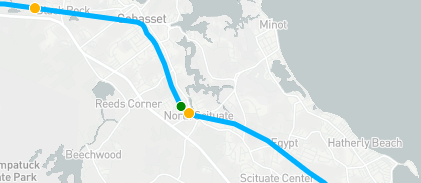
\includegraphics[width=0.4\textwidth]{prozess/animate_one_vehicle}
      \caption{Interpolation eines Vehicles entlang seiner Polyline}
      \label{fig:prozess/animate_one_vehicle}
    \end{center}
  \end{figure} 

  Das Ergebnis lässt sich in Abbildung \ref{fig:prozess/animate_one_vehicle} betrachten. Das Vehicle wird als grüner und die Stationen als orangene Kreise dargestellt.
  
% subsection animieren_eines_vehicles_durch_interpolation (end)
    \subsection{Zeichnen aller Polylines}
\label{sub:zeichnen_aller_polylines}
  Nachdem auf der Karte nun ein einzelner Trip angezeigt und animiert werden kann, sollte nun versucht werden, alle Polylines der Trips auf der Karte anzuzeigen. Abbildung \ref{fig:prozess/draw_all_shapes} zeigt, wie dies für das Boston MBTA-Feed aussieht.

  \begin{figure}[htbp]
    \begin{center}
      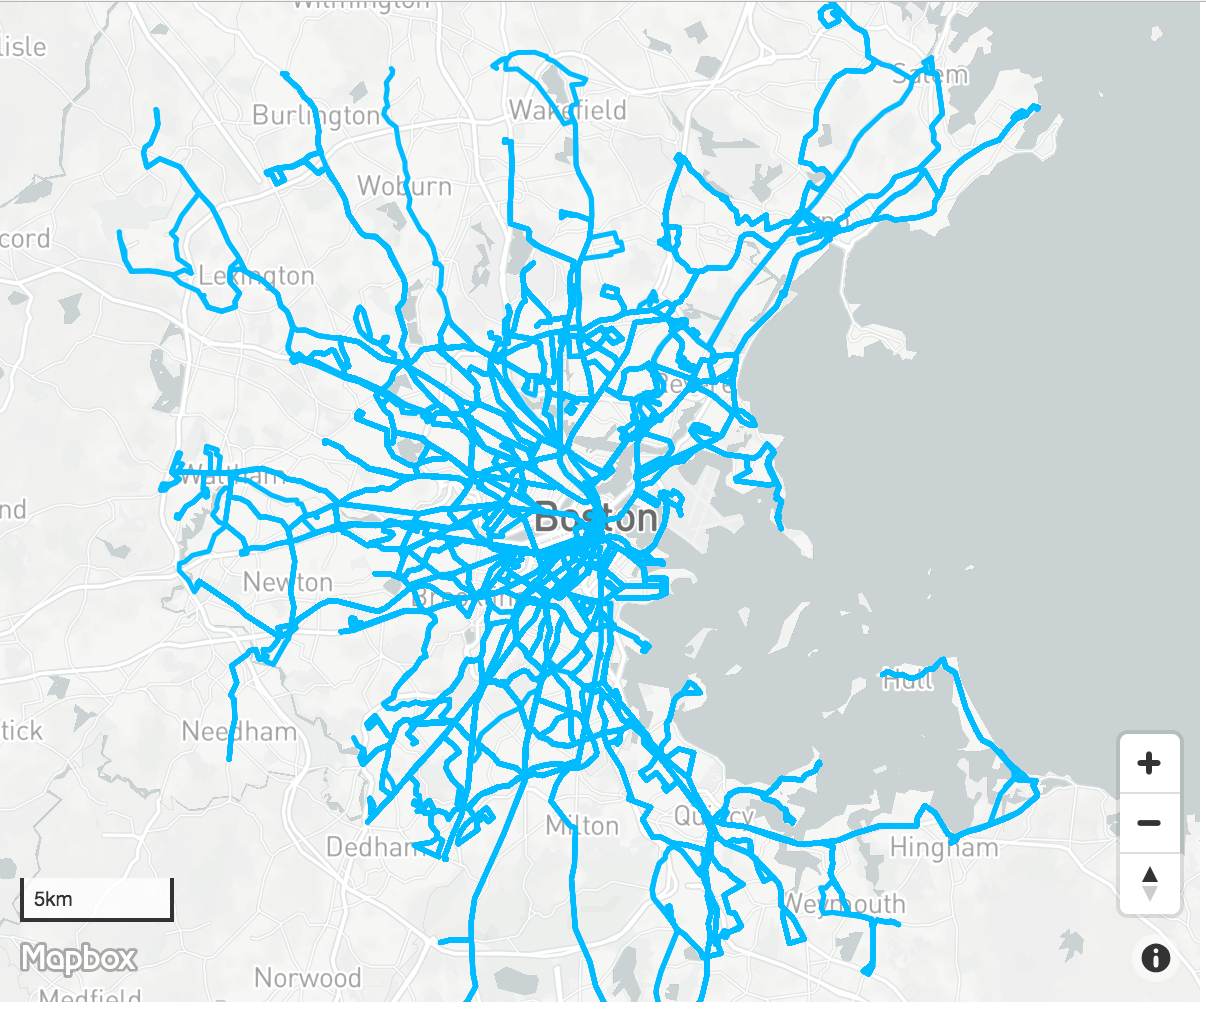
\includegraphics[width=0.5\textwidth]{prozess/draw_all_shapes}
      \caption{Darstellung aller Polylines auf der Karte}
      \label{fig:prozess/draw_all_shapes}
    \end{center}
  \end{figure}
  
  Zwar konnten alle Polylines auf der Karte angezeigt werden, allerdings bei sehr langer Rechen- und Ladezeit. Durch die Erhöhung der in der Datenbank abzufragenden Datenmenge, wurden neue Probleme offengelegt. Die ursprüngliche Datenrepräsentation der Polylines in der Datenbank war nicht optimal und die Daten ließen sich nicht performant genug abfragen. Im Folgenden sollen die Optimierungsmaßnahmen, welche an der Polyline und der Datenbank zur Steigerung der Performanz unternommen wurden, aufgezeigt werden.

  \subsubsection{Ramer–Douglas–Peucker}
  \label{ssub:ramer_douglas_peucker}
    Das Problem: Die im Stuttgart-VVS-Feed zur Verfügung gestellten Polylines sind überdefiniert und können aus tausenden Punkten bestehen. Für eine Visualisierung ist eine solche Genauigkeit nicht notwendig und aufgrund der großen Datenmenge problematisch. Durch die Verwendung des "`Ramer–Douglas–Peucker"' (RDP)-Algorithmus kann die Anzahl der Punkte einer Polyline drastisch reduziert werden. Der Vorteil besteht darin, dass dabei nicht der Linienverlauf verändert wird. Abbildung~\ref{fig:simplify} zeigt ein Beispiel einer solchen Vereinfachung mittels einer JavaScript Bibliothek\footnote{Simplify.js \url{http://mourner.github.io/simplify-js/}}.

    \begin{figure}[htbp]
      \centering
      \subfloat[Polyline vor RDP]{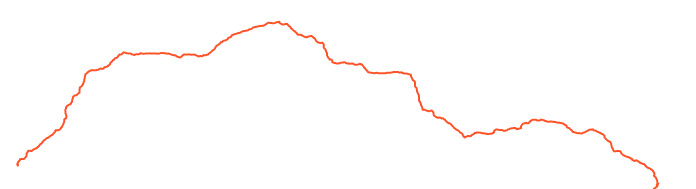
\includegraphics[width=0.48\textwidth]{simplify_before.jpg}\label{fig:simplify_before}}
      \hfill
      \subfloat[Polyline nach RDP]{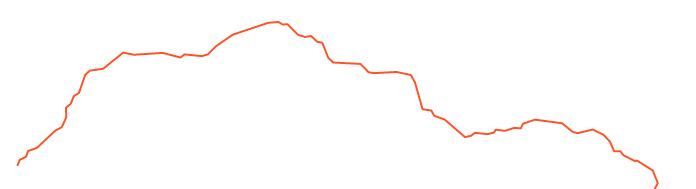
\includegraphics[width=0.48\textwidth]{simplify_after.jpg}\label{fig:simplify_after}}
      \caption{Vereinfachung einer Polyline mittels Simplify.js}
      \label{fig:simplify}
    \end{figure}

    Ausgangspunkt ist eine Polyline mit $\approx1000$ Punkten (\ref{fig:simplify}a). Nach der Vereinfachung (\ref{fig:simplify}b) ist die Anzahl auf 100 Punkte reduziert, ohne dabei visuell merklich einzubüßen. Dies ist eine erhebliche Reduzierung der Punkte um 90\%. Wie wirkt sich dieser Algorithmus positiv auf das Projekt aus? Die Vorteile sind weitreichend. Sehen wir uns die Shape-Tabelle in Abbildung \ref{fig:shape_simplify} an. \ref{fig:shape_simplify}a zeigt 394 Reihen vor der Optimierung und nur noch 140 (\ref{fig:shape_simplify}b) nach Anwendung des RDP Algorithmus.

    \begin{figure}[htbp]
      \centering
      \subfloat[Shape-Tabelle vor RDP]{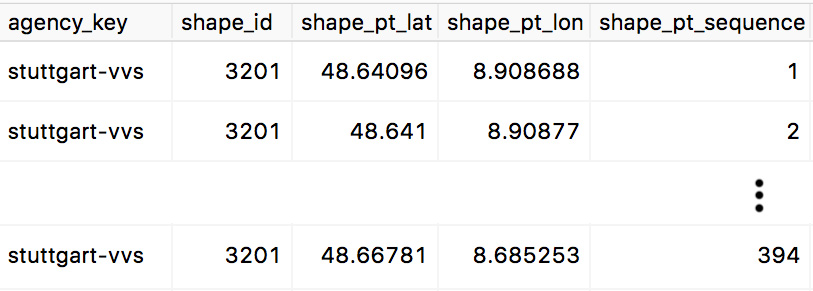
\includegraphics[width=0.48\textwidth]{shape_simplify_before.jpg}\label{fig:shape_simplify_before}}
      \hfill
      \subfloat[Shape-Tabelle nach RDP]{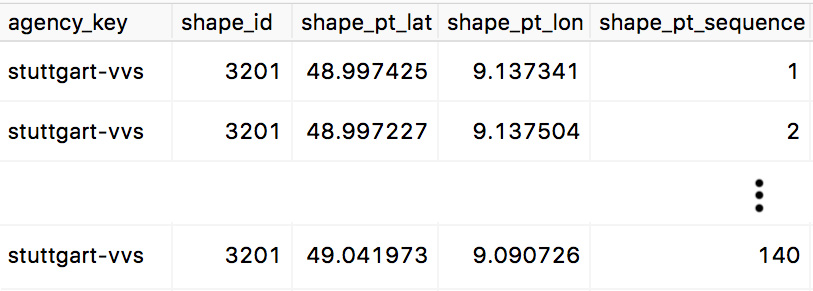
\includegraphics[width=0.48\textwidth]{shape_simplify_after.jpg}\label{fig:shape_simplify_after}}
      \caption{Reduzieren der Anzahl an Tabellen-Einträge via RDP}
      \label{fig:shape_simplify}
    \end{figure}

    In seinem Originalzustand hat das verwendete VVS-Feed 1,085,859 Mio. Zeilen. Nach der Anwendung sind diese auf 617,653 Tsd. verringert. Testet man folgende PostgreSQL Abfrage,
    \colorbox{materialGrey}{\texttt{\color{white}{{\color{materialBlue}SELECT} * {\color{materialBlue}FROM} gtfs\_shapes {\color{materialBlue}WHERE} shape\_id = {\color{materialRed}3201}}}}
    die alle Punkte einer Polyline ausgeben soll, so ergibt sich für ein optimiertes Feed eine Query-Zeit von $\approx145 ms$ und für das nicht optimierte Feed $\approx250 ms$. Schon durch diese einfache Methode sind bereits erste Performance-Steigerungen wahrnehmbar.\\

    Der RDP-Algorithmus wurde auf das GTFS-Feed angewendet, noch bevor die Daten der Polyline in die Datenbank importiert wurden. Dadurch muss die Polyline nicht während der Laufzeit vereinfacht werden, sodass diese Rechenzeit eingespart werden kann. In Kapitel \ref{ssub:gtfs_optimierungen} wird ein Tool namens \texttt{gtfstidy} vorgestellt, das GTFS-Feeds optimieren kann. Dabei ist auch das Vereinfachen von Polylines mittels RDP möglich.

  % subsubsection ramer_douglas_peucker (end)

  \subsubsection{Aggregieren der Shape-Tabelle}
  \label{ssub:aggregieren_der_shape_tabelle}
    In GTFS wird für jeden Punkt einer Polyline eine Reihe in der Datenbank belegt. Diese Abfolge ist durch eine sogenannte \texttt{Shape Point Sequence} festgelegt, was nichts anderes ist, als eine Zahl von $1$ bis $n$. Dies ist auch bereits in obiger Tabelle \ref{fig:shape_simplify} zu sehen gewesen. Sehr viel effektiver wäre es allerdings, diese Punkte nicht Reihenweise, sondern alle zusammengehörenden Punkte in nur einem einzigen Feld zu speichern. Dies ist in PostgreSQL durch eine Aggregierung möglich. Daraus ergibt sich folgende Shape-Tabelle:\\

    \begin{figure}[htbp]
      \begin{center}
        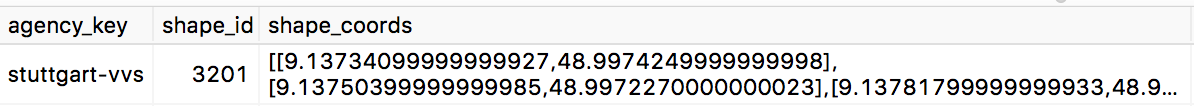
\includegraphics[width=\textwidth]{aggregated.png}
        \caption{Aggregierte Koordinaten der Shape-Tabelle}
        \label{fig:aggregated}
      \end{center}
    \end{figure}

    Wie zu sehen ist, benötigt nun eine Polyline in der Shape-Tabelle nicht mehr 140 Reihen, sondern nur noch eine einzige. Für diese Arbeit ist dies auf alle Polylines angewendet worden und in einer neuen Tabelle namens \texttt{denormalized\_shapes} abgespeichert. Dadurch ist die Berechnung der Aggregierung nur einmal nötig. Der SQL-Befehl dafür ist dem Anhang unter \ref{lst:sql_aggregate_shape} zu entnehmen.
    Wir wenden die selbe SQL-Abfrage, die bereits oben Verwendung fand, auf die neue \texttt{denormalized\_shapes} Tabelle an. Die Query-Zeit ist auf $\approx1ms$ gesunken. Anstatt hunderte Reihen, muss nur eine einzige Reihe ausgelesen werden, was sehr effizient ist. Durch das Denormalisieren\footnotemark der Shape-Tabelle ist auch die Anzahl der Reihen in der Datenbank auf ein Minimum gesunken. Von den früheren 617,653 Tsd. Reihen sind durch die Aggregation nur noch 4,524 Tsd. übrig.

    \footnotetext{Denormalisieren beschreibt den Prozess der Relationsauflösung von Datenbanktabellen.}
  
  % subsubsection aggregieren_der_shape_tabelle (end)

  \subsubsection{Polyline Encoding}
  \label{ssub:polyline_encoding}
    Die letzte Maßnahme zur Optimierung der Polyline stellt das sogenannte Polyline-Encoding dar. Wie dieses Verfahren genau funktioniert, geht an dieser Stelle zu weit. Hier soll nur erklärt werden, was unter Polyline-Encoding verstanden wird und warum es hier angewandt wird.\\

    Das Polyline-Encoding kann in JavaScript beispielsweise durch das Google-Polyline\footnote{\url{https://www.npmjs.com/package/google-polyline}} Paket eingesetzt werden. Das Encoding wandelt eine Polyline, bestehend aus Punkten, in einen String um. Zum Beispiel die Punkte: (38.5, -120.2), (40.7, -120.95), (43.252, -126.453) werden als
    \colorbox{materialGrey}{\texttt{\color{white}{\_p\textasciitilde iF\textasciitilde ps|U\_ulLnnqC\_mqNvxq`@}}}
    codiert. Dies geschieht in meiner Anwendung immer bevor Daten vom Server in Richtung Client geschickt werden: Encode $\rightarrow$ Send $\rightarrow$ Decode. Da eine codierte Polyline weniger Zeichen benötigt, kann damit Datenvolumen bei der Kommunikation zwischen Server und Client gespart werden.

  % subsubsection polyline_encoding (end)
% subsection zeichnen_aller_polylines (end)
    \subsection{Anzeigen aller Stationen}
\label{sub:anzeigen_aller_stationen}

  Nachdem zuvor alle Trips mit ihren Polylines in der Karte angezeigt wurden, folgt nun das Anzeigen aller Stationen, die zu einem Trip gehören. Änlich wie beim Abfragen und Anzeigen aller Polylines, sollte dieser Schritt mögliche Engpässe oder unvorhergesehene Probleme aufdecken (Abbildung \ref{fig:prozess/draw_all_stations}).

  \begin{figure}[htbp]
     \begin{center}
       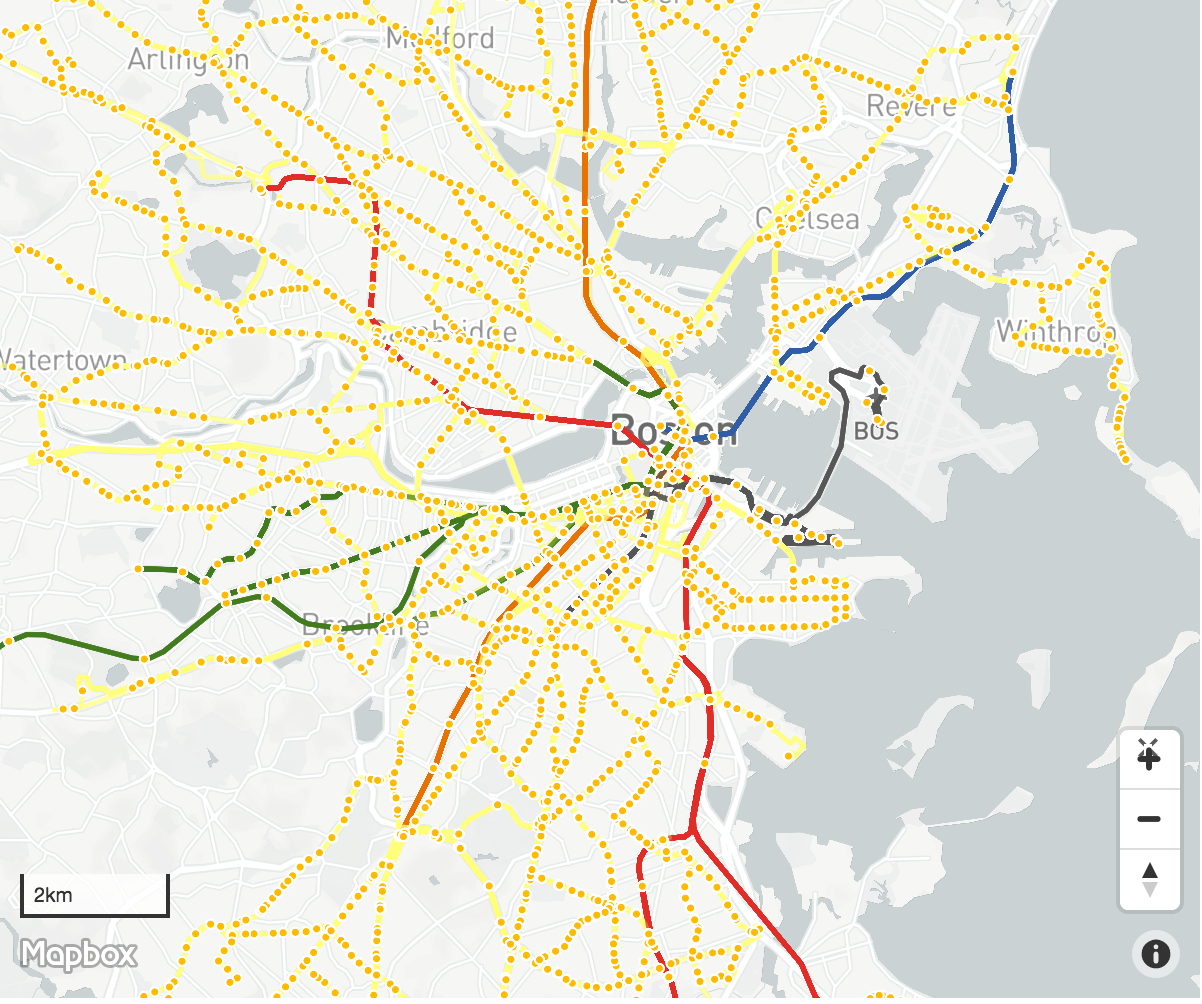
\includegraphics[width=0.6\textwidth]{prozess/draw_all_stations}
       \caption{Aktive Trips mit ihren dazugehörenden Stationen}
       \label{fig:prozess/draw_all_stations}
     \end{center}
   \end{figure}
   
  Vor allem die Abfrage von aktiven Trips aus der Datenbank, stellte ein großes Problem dar. Die Datenbank konnte die Anfragen des Clients nicht effizient genug verarbeiten. An dieser Stelle stand fest, dass für die weitere Arbeit umfassende Optimierungen der Datenbank erfolgen müssen, um eine responsive Webanwendung zu ermöglichen. 

  \subsubsection{GTFS Optimierungen}
  \label{ssub:gtfs_optimierungen}
    Der erste Schritt um die Performance zu verbessern, ist die Optimierung von GTFS Feeds. Damit lässt sich die Datenmenge bereits vor dem Importieren in die Datenbank, erheblich verringern. Ein Tool um ein GTFS Feed umfassend zu optimieren ist \texttt{gtfstidy} \url{https://github.com/patrickbr/gtfstidy}. Es bietet dabei allerdings nicht nur die Möglichkeit für die Vereinfachung von Polylines sondern kommt mit einer ganzen Reihe an Optimierungsmöglichkeiten. 

    Der Kommandozeilenbefehl \colorbox{materialGrey}{\texttt{\color{white}{\$ gtfstidy -sSiRDeO input.zip output}}} optimiert das Stuttgart-VVS Feed wie folgt:
    
    \begin{itemize}[label={}]
      \item \textbf{-s} Reduziert die Punktanzahl einer Polyline
        
      \item \textbf{-S} Entfernt redundante Polylines.

      \item \textbf{-i} Umwandlung von Zeichen ID's (String) in Zahlen ID's (Integer).\footnote{Aus der String ID \texttt{'1.T0.10-1-j17-1.16.H'} wird \texttt{78}}

      \item \textbf{-O} Entfernt Feed Einträge die nicht referenziert werden.

      \item \textbf{-R} Entfernt doppelt vorhandene Routen.

      \item \textbf{-e} Setzt fehlerhafte oder optionale Felder auf einen Standard Wert.

      \item \textbf{-D} Entfernt fehlerhafte Einträge aus dem Feed.
    \end{itemize}

    Durch Verwendung von gtfstidy konnte das Feed optimiert werden und die Datengröße der einzelnen Dateien um folgendes Maß verringert werden.

    \begin{longtable}{|>{\raggedright \arraybackslash}p{5.0cm}|>{\raggedright \arraybackslash}p{5.0cm}|>{\raggedright \arraybackslash}p{5.0cm}|}
      \hline
      Dateiname & Größe davor& Größe danach\\
      \hline
      trips.txt & 6 MB & 2.8 MB\\
      stop\_times.txt & 103 MB & 53 MB\\
      stops.txt & 651 KB & 355 KB\\
      shapes.txt & 77.3 MB & 22.4 MB\\
      routes.txt & 54 KB & 38 KB\\
      calendar\_dates.txt & 557 KB & 463 KB\\
      \hline
      \caption{Tabellengröße bevor und nach anwenden von gtfstidy}
      \label{tbl:gtfs_tidy_results}
    \end{longtable}

    Insgesamt konnte so die Größe des Feeds von 79 MB auf 118 MB um knapp 50\% verringert werden. Vor allem die Umwandlung von langen String ID's in kürzere Integer ID's trägt maßgeblich zur Verringerung der Dateigröße bei.

  % subsubsection gtfs_optimierungen (end)

  \subsubsection{Denormalisierung der Datenbank}
  \label{ssub:denormalisierung_der_datenbank}
    Die Denormalisierung ist eine Strategie, die auf eine zuvor normalisierte Datenbank angewendet wird, um die Leistung zu erhöhen. Die Denormalisierung ist der Prozess, bei dem versucht wird, die Leseperformance einer Datenbank zu verbessern, auf Kosten der Schreibleistung, durch Hinzufügen redundanter Kopien von Daten oder durch deren Gruppierung.\parencite{sanders}
    Der große Nachteil von Denormalisierung, nämlich die Redundanz von Daten, spielt für dieses Projekt keine Rolle, da die Daten ausschließlich ausgelesen und nicht geschrieben werden. Was bleibt sind die Vorteile.\\

    Für dieses Projekt bedeutet diese Methode, eine neue Tabelle zu generieren, die den Zugriff auf die benötigten Daten einfach macht. Im Grunde handelt es sich um eine Vorberechnung. Anstatt die Tabellen bei jeder Anfrage an den Server aufwendig über viele \texttt{SQL-JOINS} zu verknüpfen, wird diese Verknüpfungen einmalig vorberechnet und in eine Tabelle gespeichert. Eine Denormalisierung  einer Tabelle ist bereits im vorherigen Abschnitt "`\nameref{ssub:aggregieren_der_shape_tabelle}"' gezeigt und führte dazu, dass die Polyline über die Abfrage einer einzigen Tabellenreihe erhalten werden kann was die Performance signifikant erhöhte. Zur besseren Verständnis soll folgende Grafik helfen:

    \begin{figure}[htbp]
      \begin{center}
        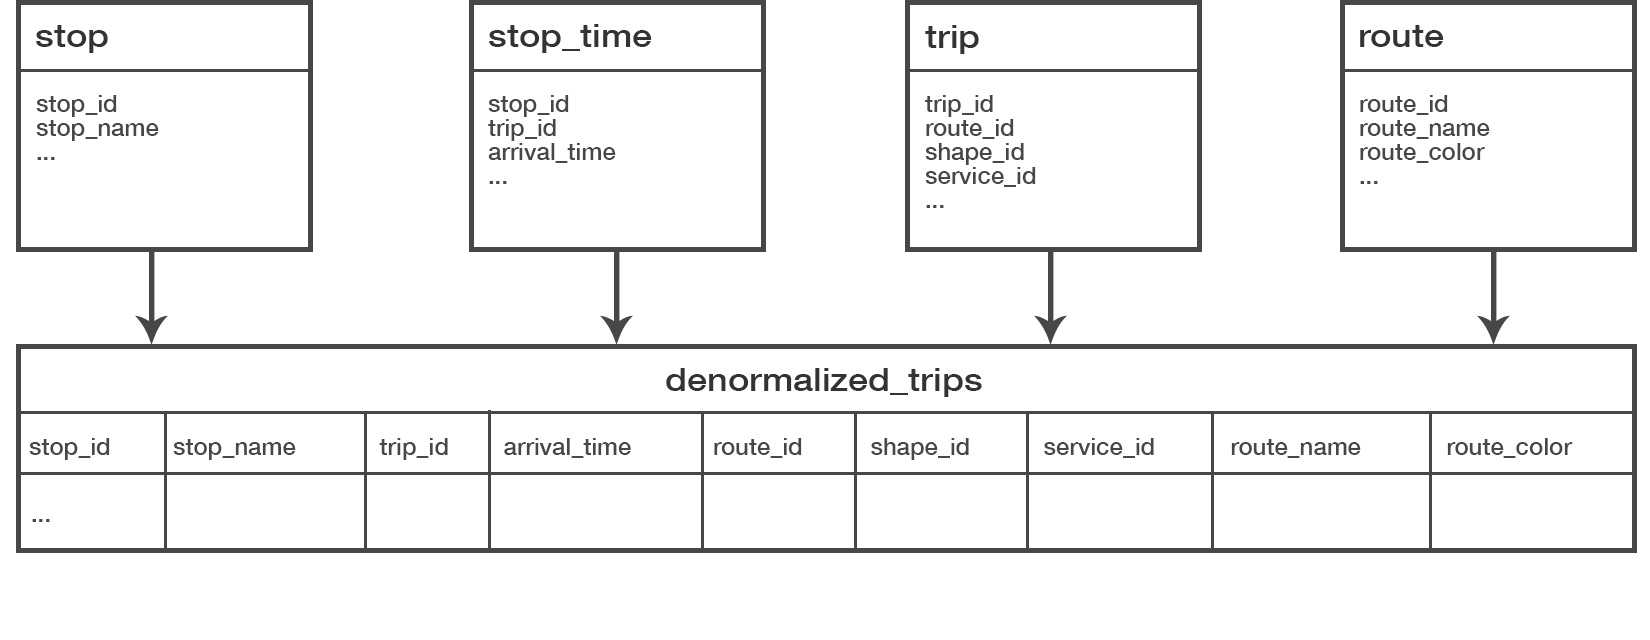
\includegraphics[width=\textwidth]{denormalizing.jpg}
        \caption{Beispiel einer Denormalisierung von Tabellen}
        \label{fig:denormalizing}
      \end{center}
    \end{figure}

    Wie in Abbildung \ref{fig:denormalizing} zu sehen ist, wird aus einer vertikalen Anordnung der einzelnen Datenfelder, eine horizontale Anordnung in einer einzigen \texttt{denormalized\_trips} Tabelle. Eine Reihe in dieser neuen Tabelle steht für genau einen Eintrag eines Trips. Anstatt also bei jeder Anfrage an den Server die verschiedenen Daten mittels \texttt{JOIN} verknüpfen zu müssen, können diese jetzt per Zugriff auf eine einzige Reihe in nur einer Tabelle erfragt werden.

    Dieses Prinzip, der Gruppierung von Daten in einer neuen Tabelle soll nun auch auf die anderen benötigten Tabellen angewendet werden. Die Denormalisierung erfolgt in 3 Schritten:

    \begin{enumerate}
      \item Erstellen der neuen Tabelle \texttt{denormalized\_trips}
      \item Importieren der verschiedenen Daten in diese neue Tabelle
      \item Mögliche Abfragen sind nun über diese neue Tabelle möglich.
    \end{enumerate}

    Das SQL-Statement ist abermals aufgrund seiner Länge Anhang \ref{lst:denormalized_shapes} zu entnehmen. Dies resultiert in einer Tabelle die wie folgt aussieht:

    \begin{figure}[htbp]
      \begin{center}
        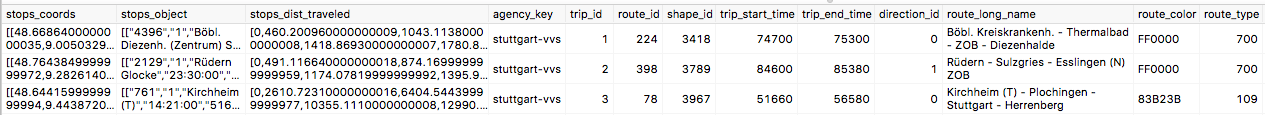
\includegraphics[width=\textwidth]{denormalized_tables.png}
        \caption{Auszug aus der \texttt{denormalized\_trips} Tabelle}
        \label{fig:denormalized_table}
      \end{center}
    \end{figure}  

    \subsubsection*{Ergebnisse der Denormalisierung}
    \label{ssub:ergebnisse_der_denormalisierung}
      Für die Visualisierung ist eine Abfrage der aktiven Trips am wichtigsten.
      Folgende Tabellen werden für die Abfrage benötigt.

      \begin{figure}[htbp]
        \begin{center}
          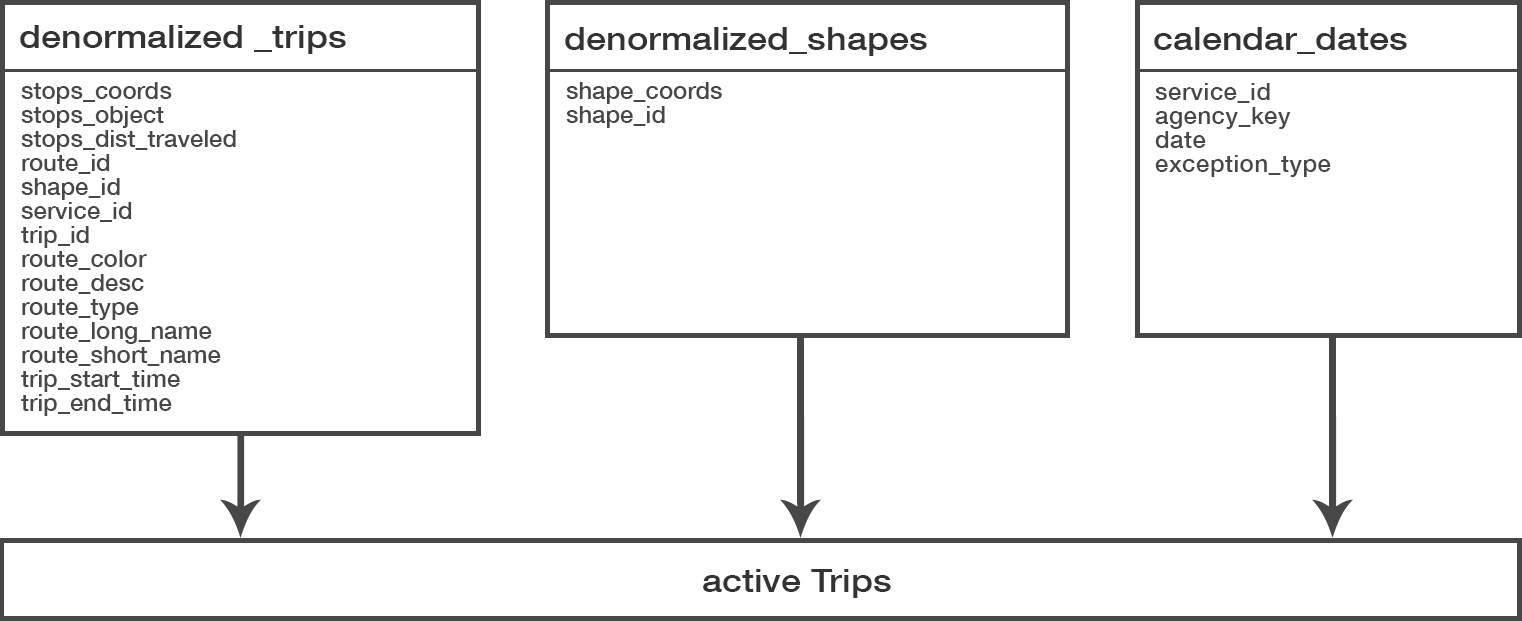
\includegraphics[width=\textwidth]{denormalizing_results.jpg}
          \caption{Benötigte Tabellen zur Abfrage von Trips}
          \label{fig:denormalizing_results}
        \end{center}
      \end{figure}

      Wie zu sehen ist, wird auf die Denormalisierte \texttt{Shape} und \texttt{Trips} Tabelle zugegriffen.

      Nachfolgend die Ergebnisse für die Abfrage von Trips in einem wachsenden Zeitrahmen. Die verwendete SQL-Abfrage befindet sich im \nameref{sec:anhang} unter Listing \ref{lst:query_trips}.

      \begin{longtable}{|>{\raggedright \arraybackslash}p{5.0cm}|>{\raggedright \arraybackslash}p{5.0cm}|>{\raggedright \arraybackslash}p{4.0cm}|}
      \caption{Evaluierung der Denormalisierung}\label{tbl:evaluierung_der_denormalisierung}\\
        \hline
          Zeitraum & Trip Anzahl & Query Zeit\\
        \hline
          9:00 bis 9:15 & 88 & 98 ms\\
          9:00 bis 10:00 & 1125 & 154 ms\\
          9:00 bis 12:00 & 3360 & 285 ms\\
          9:00 bis 15:00 & 7070 & 497 ms\\
          9:00 bis 21:00 & 14718 & 900 ms\\
        \hline
      \end{longtable}

      Die Ergebnisse Zeigen, dass die Abfragezeit der Datenbank für die aktiven Trips erheblich gesunken ist. Anfangs ist solch eine Anfrage aufgrund der endlosen Laufzeit erst gar nicht möglich gewesen.

      \begin{figure}[htbp]
        \begin{center}
          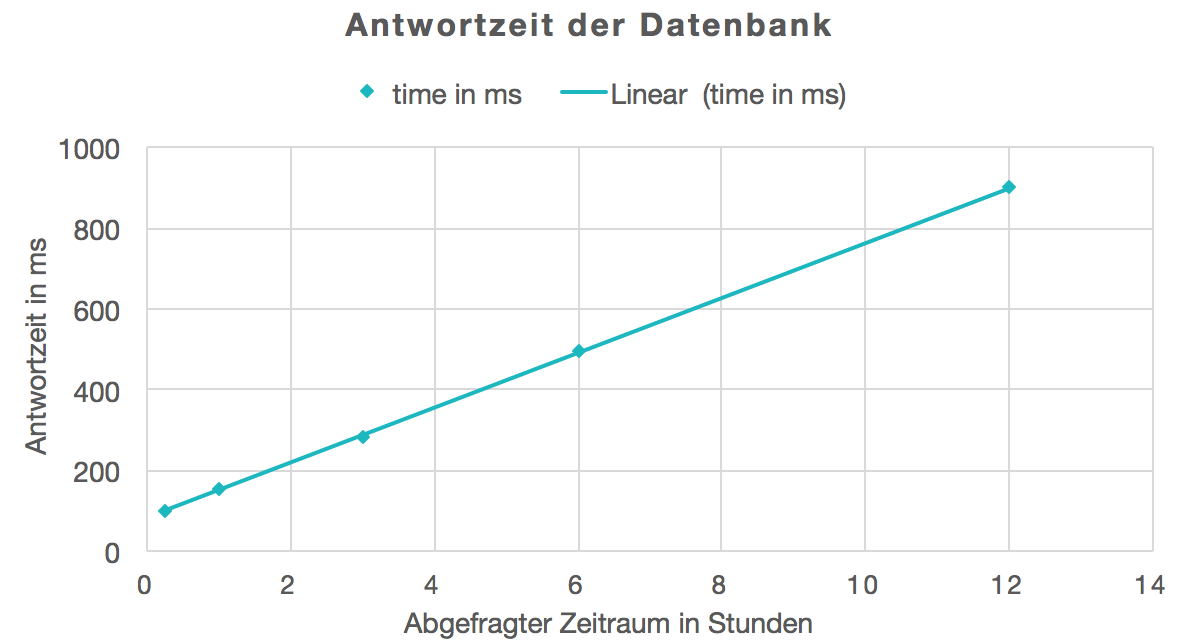
\includegraphics[width=0.7\textwidth]{query_time_chart}
          \caption{Plot der Abfragezeiten}
          \label{fig:query_time_chart}
        \end{center}
      \end{figure}
      
      Abbildung \ref{fig:query_time_chart} zeigt einen Plot der Query Zeit aus Tabelle \ref{tbl:evaluierung_der_denormalisierung} als linearen Graphen. Daraus folgt, dass die Antwortzeit der Datenbank linear mit dem abgefragten Zeitraum wächst. Für die Visualisierung sind vor allem zwei Abfragen wichtig: Erstens das Abfragen eines größeren Zeitraums von 1-2 Stunden. Dies geschieht beim ersten Aufrufen der Webanwendung wenn die Karte noch keine Trips besitzt und damit leer ist. Zweitens die Abfrage von nur kleinen Zeiträumen von nur einer Minute, um neue Trips abzufragen. Für diese zwei Abfragen bewegt sich die Antwortzeit des Servers zwischen $\approx 80 -  160\; ms$. Damit wurde das in Kapitel \ref{sub:zielsetzung} gesetzte ziel von 0 bis $200ms$ bereits erreicht.
      
    % subsubsection ssub:ergebnisse_der_denormalisierung (end)
  % subsubsection denormalisierung_der_datenbank (end)
% subsection anzeigen_aller_stationen (end)
    \subsection{Animieren der aktiven Trips}
\label{sub:animieren_der_aktiven_trips}
  Nachdem die Daten für alle aktiven Trips im Client ankommen, kann für jeden Trip ein Vehicle erstellt werden. In einem Animation-Loop wird für jedes Vehicle pro Frame, eine neue Position berechnet und die Karte wird mit der neuen Position aktualisiert. Der Algorithmus dafür ist in Pseudo-Code in Listing \ref{alg:animate_algorithmus} beschrieben.

  \begin{algorithm}[H]
    \caption{Animate Vehicle}\label{alg:animate_algorithmus}
    \begin{algorithmic}[1]
      \Procedure{animateVehicle}{}
        \State ServerQueryTimer $\gets$ 30 Seconds
        \State Vehicles $\gets$ Vehicles Inside Bounding Box
        \State Trips $\gets$ Requested Trips
        \Function{animate}{timestamp}
          \ForAll{Vehicles as Vehicle} \State{
            \If{Vehicle started its Trip} 
              \State \Call{calculateVehiclePosition}{Vehicle}
            \EndIf
            \If{Vehicle not started its Trip}
              \State \Call{checkVehicleActivity}{Vehicle, Trips}
            \EndIf
            \State \Call{checkIfVehicleHasFinished}{Vehicle}
            \State \Call{updateMapWithNewPositions}{Vehicles}
          }\EndFor

          \If{ServerQueryTimer Expired} 
            \State Query Server for New Trips
            \State ServerQueryTimer $\gets$ 30 Seconds
          \EndIf

          \State \Call {animate}{timestamp}
        \EndFunction
        
      \EndProcedure
    \end{algorithmic}
  \end{algorithm}

  Innerhalb dieses Animation-Loops passieren mehrere Dinge. Zuerst wird geprüft ob sich ein Vehicle überhaupt im Sichtbereich des Anwenders befindet. Trifft das zu, wird für eben diese Vehicle die Distanzen berechnet und die Position des Vehicles entlang der Polyline interpoliert. Falls das Vehicle seinen Trip noch nicht begonnen hat, wird überprüft ob das immer noch der Fall ist. Anschließend werden alle Vehicle geprüft, ob sie ihren Trip erledigt haben. Danach wird die Karte mit den neuen Positionen der Vehicle aktualisiert. Während all dies geschieht, läuft ein Timer mit, der nach dem Ablaufen von 30 Sekunden den Server nach neuen Trips abfrägt.

  Das Ergebnis ist die Animation aller Vehicle der momentan aktiven Trips (Abbildung \ref{fig:prozess/animate_all_vehicles}).

  \begin{figure}[htbp]
    \begin{center}
      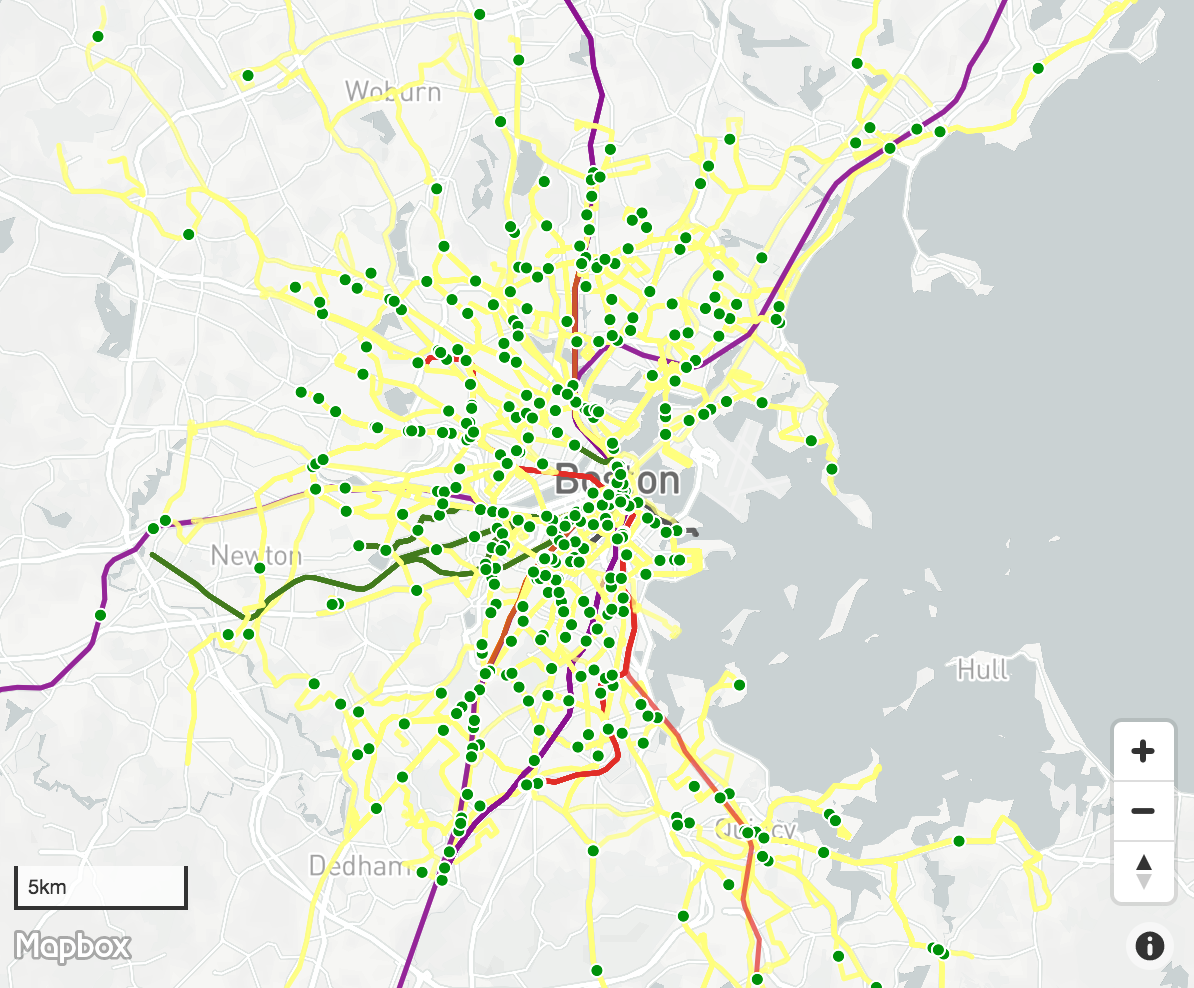
\includegraphics[width=0.7\textwidth]{prozess/animate_all_vehicles}
      \caption{Animieren aller Vehicles auf der Karte}
      \label{fig:prozess/animate_all_vehicles}
    \end{center}
  \end{figure}
  
  
  
% subsection animieren_der_aktiven_trips (end)

  % section develop (end)
\end{newpage}